\chapter{Error Measures}\label{sec:error}
To be able to compare different statistical models some kind of performance 
measure, usually in the form of an error measure, is needed. In the plume 
modelling task one is interested in the deviation of the predicted mean 
concentrations $\mu(\vc x)$ from the true ones $c(\vc x)$. When using the $L^2$ 
norm and integrating over the complete task volume $V$ the \newtermAbbrev{root 
    mean integrated square error}{RMISE}
\begin{equation}
    E\ped{RMISE} = \sqrt{\frac{1}{v} \int_V \del{c(\vc x) - \mu(\vc x)}^2 
        \dif\vc x}
\end{equation}
with
\begin{equation}
    v = \int_V \dif\vc x
\end{equation}
is obtained. However, it can be assumed that accurate predictions are more 
important where the concentrations is actually high 
\parencite[c.p.][]{Marchant:2012wb}. Thus, it might be beneficial to introduce 
a weighting factor $w(\vc x)$ to
\begin{equation}
    E\ped{WRMISE} = \sqrt{\frac{1}{v} \int_V \del{c(\vc x) - \mu(\vc x)}^2 w(\vc 
        x) \dif\vc x} \text{,}
\end{equation}
the \newtermAbbrev{weighted root mean integrated square error}{WRMISE}, with
\begin{equation}
    w(\vc x) = \frac{c(\vc x) - \min c(\vc x')}{\max c(\vc x') - \min c(\vc x')} 
    \text{.}
\end{equation}
Note that in areas with concentration of almost or even exactly zero the WISE 
will always be close to zero and thus allowing the model to make highly 
inaccurate predictions. Therefore, the WISE should not be used as sole measure 
in plume modelling. Using both errors it is possible to ensure good overall fit 
of the prediction without large inaccuracies and to compare which model has the 
better fit in the interesting areas.

Unfortunately, the RMISE and WRMISE cannot easily be calculated analytically and 
one has to restrain to approximating the integral from a finite set $\{\vc x_i 
| i = 1, \dots, n\}$ of samples. If the $x_i$ are distributed according to the 
probability density function $p(\vc x)$, the approximation has the form
\begin{align}
    \hat E\ped{RMISE} &= \sqrt{\frac{1}{vZ} \sum_{i=1}^n \frac{\del{c(\vc x_i) 
                - \mu(\vc x_i)}^2}{p(\vc x_i)}} \\
    \hat E\ped{WRMISE} &= \sqrt{\frac{1}{vZ} \sum_{i=1}^n \frac{\del{c(\vc x_i) 
                - \mu(\vc x_i)}^2 w(\vc x_i)}{p(\vc x_i)}} \text{.}
\end{align}
The normalization constant $Z$ is given by
\begin{equation}
    Z = \sum_{i=1}^n \frac{1}{p(\vc x_i)} \text{.}
\end{equation}

The probability density $p(\vc x)$ can be estimated using Gaussian 
\abbrev{kernel density estimation}{KDE}. There exist different methods to 
determine the bandwidth parameter of the KDE\@. In this work Scott's Rule 
\parencite{Scott:2009tl} was used.

\section{Selecting Samples for Error Approximation}\label{sec:mh}
Up to now it is still open how to select the $x_i$ for approximating the error 
measures.  Using a regularly spaced grid is either likely to miss the important 
areas as the plume is quite localized or it is so fine grained that the 
evaluation of the error takes a long time. Thus, I used a slightly modified 
\abbrev{Metropolis-Hastings}{MH} algorithm to concentrate samples in areas with 
a high concentration.

The standard Metropolis-Hastings \parencite{Chib:1994ud} is used to sample from 
a probability distribution $P(\vc x)$ given only a function $f(\vc x)$ 
proportional to $P(\vc x)$. It starts at a random location $\vc x_1$.  Then in 
each iteration $i > 0$ a new candidate location $\vc x_*$ is picked from 
a symmetric\footnote{$Q(\vc a | \vc b) = Q(\vc b | \vc a)$} proposal 
distribution and an acceptance ratio $\xi = f(\vc x_*) / f(\vc x_i)$ is 
calculated. The candidate $\vc x_*$ is accepted as $\vc x_{i + 1} = \vc x_*$ 
with probability $\xi$ ($\xi \geq 1$ automatically accepts). If it is rejected, 
$\vc x_{i + 1} = \vc x_i$ will be used.

To select the samples for the error approximation this algorithm can be used 
with the true concentrations $f(\vc x) = c(\vc x)$. For this purpose it is not 
necessary that the samples exactly follow a specific probability distribution.  
That makes it possible to make a few adoptions for better results.

First of all, $\vc x_*$ can always be added to the set of samples independent of 
acceptance or rejection instead of the accepted sample.  This makes each 
location unique (as long as the same location does not get proposed twice).  
Having multiple instance of the same location within the samples would not 
increase the accuracy of the error approximation. Also, this leads to a few more 
samples towards the concentration tails where the concentration is already low 
but spatially close to high concentrations.  Thus, the approximation around the 
concentration slope can be expected to be better.

A further change concerns the initial location $\vc x_1$. Choosing at randomly 
might place it in an area with zero concentration which renders the acceptance 
ratio $r$ undefined. Hence, it is better base the initial location on the source 
locations. Unfortunately, given a plume dispersion 
(Equation~\ref{eqn:plumedisp}) the plume concentration is undefined at the 
source location. To circumvent this, the initial location $\vc x_1$ should be 
excluded from the samples.

In case of multiple sources it should be started from each source location and 
the resulting sets should be joined. The concentration between sources can be 
rather low making it unlikely to switch from one plume to another. Also, the 
Metropolis-Hastings algorithm is unlikely to sample in low concentration areas, 
especially in some distance to the plumes. Thus, a number of uniformly sampled 
locations should be added.

To ``smooth'' out the samples around the plumes even more one can use only every 
$k$-th sample of the Metropolis-Hastings algorithm and use the remaining samples 
as center of Gaussian distributions and draw $k$ more samples from each of 
these.

\section{QRSim Reward}\label{sec:qrsim-reward}
The plume modelling scenarios in \textcite{denardi2013rn} themselves define 
a reward
\begin{equation}
    R = - \sum_{i = 1}^n \del{c(\vc x) - \mu(\vc x)}^2
\end{equation}
as a performance measure. This is essentially the negative of 
$\hat{E}\ped{RMISE}^2$ without normalization. Thus, with a non uniform sampling 
this reward will give a biased estimate attributing more importance to areas 
with more sample locations.

The set of $\vc x_i$ used to calculate the reward in QRSim consists ouf of two 
parts. One-fifth is sampled uniformly over the whole volume whereas the 
remaining samples are taken uniformly from the areas where the concentration 
exceeds the limit $c_{\min} = Q \cdot 10^{-3} \cdot 
\si{\second\per\meter\cubed}$.

The bias introduced by that towards the interesting regions is not necessarily 
bad. The same is done in the WRMISE\@. Unfortunately, the sampling strategy will 
not sample at the low side of a (steep) concentration boundary and will give an 
bad estimate of the reward around those boundaries. In contrast to that, the 
Metropolis-Hastings based sampling algorithm acquires also some samples in the 
low concentration area around a high concentration.  This difference is 
visualized in Figure~\ref{fig:err-sampling}.

\begin{figure}
    \centering
    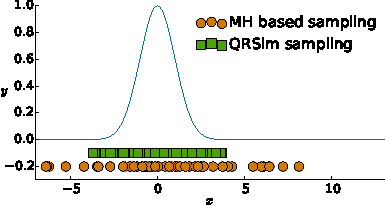
\includegraphics{plots/err-sampling}
    \caption[Comparison of error estimation sampling methods]{One-dimensional 
        comparison of the Metropolis-Hastings based sampling and the QRSim 
        sampling for error estimation. For both approaches 60 samples with 
        regard to the plotted Gaussian density were taken excluding the 
        uniformly distributed samples.  The $y$ position of the scatter marks 
        has no meaning in this plot. For the MH based sampling in this plot 
        every fifth sample was used.  A Gaussian was used as proposal 
        distribution with $\sigma = 2$.  The same distribution was used to 
        create five additional samples for each MH based 
        sample.}\label{fig:err-sampling}
\end{figure}

\section{Normalized Error}
For a reliable comparison of the models it is not sufficient to compare them 
based on a single trial. A good model should provide a low error in different 
trials.

In the plume modelling scenarios the concentration density and spatial extend of 
the plume varies. The error measures directly depend upon the absolute 
concentration values and, therefore, also depend on the specific trial.

Directly averaging the error over trials would give a higher weighting to trials 
with high concentration densities or a large plume extend. A good plume 
modelling method should adapt to the concentration levels and be more precise 
for lower overall concentrations. To achieve a fair weighting of the trials the 
error can be normalized as
\begin{equation}
    F = \frac{E}{E_0}
\end{equation}
for each trial, where $E$ is the current error estimate and $E_0$ the error 
estimate for an all zero prediction. The error estimate can be freely chosen 
with regard to its properties. Note that this equation can also be applied to 
the reward $R$ as error measure as the minus cancels out. When averaging $F$ 
over trials each trial is weighted equally.

The normalized error $F$ has also the advantage of being readily interpretable.  
For $F > 1$ the prediction is worse than an all zero prediction.  This should 
for not happen with a viable modelling method. For $F < 1$ the prediction is 
better than an all zero prediction and the error has been decreased by $(1 - F) 
\cdot \SI{100}{\percent}$.
